%%% Journal of Control and Decision (JCD) submission version.
%%% Content is identical to ../main.tex; only the class scaffolding differs.
%%%
%%% Build:  tectonic main.tex          (runs XeTeX + BibTeX automatically)
%%% or:     xelatex main / bibtex main / xelatex main / xelatex main
%%%
%%% Layout parameters come from jcd.cls and must not be altered:
%%% double column, 10.5 bp body, 20 mm margins, Times.

% Loaded before the class so that the Times font probes resolve in T1 rather
% than the engine-default TU encoding (removes spurious substitutions under
% XeTeX/tectonic).
\RequirePackage[T1]{fontenc}
\documentclass{jcd}

\usepackage[utf8]{inputenc}
\usepackage{amsmath}
% Times text and Times-compatible math, matching the class's mandated face.
% newtxmath also supplies the AMS symbol set, so amssymb must NOT be loaded.
\usepackage{newtxtext}
\usepackage[varvw]{newtxmath}
\renewcommand\sfdefault{\rmdefault}

\usepackage{graphicx}
\usepackage{booktabs}
\usepackage{multirow}
\usepackage{makecell}
\usepackage{array}
\usepackage{tabularx}
\usepackage{siunitx}
\usepackage{float}
\usepackage{xcolor}

\colorlet{url}{black}
\usepackage{hyperref}
\hypersetup{
  colorlinks = true,
  citecolor  = ref,
  linkcolor  = ref,
  urlcolor   = url,
}
\usepackage[numbered]{bookmark}

% url.sty ships a stretchable inter-character glue; in a 234 pt justified
% column that pulls a long repository URL apart into visible gaps. xurl
% already permits a break at every character, so no stretch is needed.
\Urlmuskip=0mu\relax

% Figures live one level up, alongside the IEEE version; the journal logos
% used by the class page style live next to this file.
\graphicspath{{../}{logos/}}

\sisetup{
  range-phrase = {\,--\,},
  range-units  = single,
  detect-weight = true,
  detect-family = true,
  separate-uncertainty = true,
}

% Uniform row height for the multi-line table headers used in Section 5.
\renewcommand{\theadfont}{}
\renewcommand{\cellalign}{cc}

\makeatletter
% The class puts the trailing period of a heading number inside \thesection,
% which would leak into every \ref. Move the period into the heading format so
% the printed headings are unchanged ("1.", "1.1.") while cross-references read
% "Sec. 5.1" rather than "Sec. 5.1.".
\renewcommand{\thesection}{\arabic{section}}
\renewcommand{\thesubsection}{\arabic{section}.\arabic{subsection}}
\renewcommand{\thesubsubsection}%
  {\arabic{section}.\arabic{subsection}.\arabic{subsubsection}}
\titleformat{\section}[hang]
  {\@normalspace\sffamily\large\bfseries\color{main}\raggedright}
  {\thetitle.}{.5em}{}{}
\titleformat{\subsection}[hang]
  {\@normalspace\sffamily\normalsize\bfseries\itshape\color{main}}
  {\thetitle.}{.5em}{}{}
\titleformat{\subsubsection}[hang]
  {\@normalspace\sffamily\normalsize\bfseries\itshape\color{main}}
  {\thetitle.}{.5em}{}{}
% The class resets the equation counter at every section but prints it without
% a section prefix, which would repeat numbers. Number equations continuously.
\counterwithout{equation}{section}
\makeatother

% The journal column is 82 mm, ~7% narrower than the IEEE one this text was
% first set in. Give the line breaker a little extra slack so that unbreakable
% tokens (\path{}, \SIrange{}) do not force overfull lines.
\setlength{\emergencystretch}{3em}

% Float placement. The source was set for a 252 pt IEEE column; the journal's
% is 234 pt, so several tables grow past the height a top-only float can
% occupy. Without a float page in the allowed positions LaTeX defers such a
% float indefinitely and drops it at the end of the document, silently. Allow
% h/b/p everywhere and raise the per-page float counts so the queue drains
% near the text that cites it.
\setcounter{topnumber}{3}
\setcounter{bottomnumber}{2}
\setcounter{totalnumber}{5}
\setcounter{dbltopnumber}{3}

\renewcommand{\textfraction}{0.1}
\renewcommand{\topfraction}{0.9}
\renewcommand{\dbltopfraction}{0.9}
\renewcommand{\bottomfraction}{0.5}
\renewcommand{\floatpagefraction}{0.7}

% A float column is filled with \@fptop/\@fpsep/\@fpbot glue, all of which
% default to "0pt plus 1fil". That centres the floats vertically and opens the
% large blank bands above and below a table that lands on a float column. Pin
% the first float to the top and let the slack collect at the bottom instead.
\makeatletter
\setlength{\@fptop}{0pt}
\setlength{\@fpsep}{10pt plus 1fil}
\setlength{\@fpbot}{0pt plus 1fil}
\setlength{\@dblfptop}{0pt}
\setlength{\@dblfpsep}{10pt plus 1fil}
\setlength{\@dblfpbot}{0pt plus 1fil}
\makeatother

% Table notes: \centering (set by the table env) leaves \rightskip/\parfillskip
% at fil, which centres every last line. \tabnote restores normal justification.
% The 2em of \rightskip stretch is not cosmetic: notes carry unbreakable
% \path{} and \texttt{} filenames, and in a full-justified column those force
% badness-10000 underfull lines with visibly gaping interword space. A little
% permitted raggedness absorbs them instead.
\newcommand{\tabnote}{\par\leftskip=0pt\rightskip=0pt plus 2em%
  \parfillskip=0pt plus 1fil\relax}

\documentsetup{
  title={Anchored Conditionally-Gated Control for Wheeled Bipedal Balance and
         Disturbance Recovery},
  history={Received ***\\ Accepted ***},
  keywords={Wheeled biped robot; conditionally-gated control; anchored
            standing; proximity-gated integral; push recovery; disturbance
            rejection.},
  authors={
    Author's name={a},
  },
  affiliations={
    a={The University of Danang, Viet Nam},
  },
  short-author={Author's name},
  contact-to={Author's name},
  contact-email={Mailexample@gmail.com},
  contact-address={The University of Danang, Viet Nam.},
}

\begin{document}

\maketitlepage
\arrayrulecolor{main} % set table line color


% ============================================================
\begin{abstract}
Wheeled bipedal robots face a trade-off: the stiffness that buys precise standing shrinks the push-recovery envelope, while the integral action that removes equilibrium bias winds up during disturbances. The Anchored Conditionally-Gated Controller (ACC) answers both by \emph{conditional activation}: a position integral confined to a \SI{15}{cm} neighbourhood and enabled by an asymmetric envelope follower ($\tau_{\text{attack}}{\approx}\SI{23}{ms}$, $\tau_{\text{release}}{\approx}\SI{1.5}{s}$) that separates quiet stance from post-push ringdown. On a \num{10}-DOF, \SI{8.1}{kg} wheeled biped in MuJoCo (\SI{500}{Hz} physics, \SI{100}{Hz} control) the architecture is dissected, not only demonstrated. A factorial ablation separates three coupled effects: gated damping produces the steadiness, the anchor integral the accuracy, and the gates are bit-identical to ACC in quiet stance yet decisive under disturbance. The push envelope is measurably chiral (\SI{-17.3}{N}), traced to the antisymmetric hip-roll/hip-yaw channels. A closed-form model predicts the \SI{27.0}{mm} standing offset to \SI{0.92}{\percent} across a fortyfold gain sweep, as the price of a bounded integrator memory. ACC holds $0.294{\pm}0.015$\,mm sagittal repeatability ($N{=}10$), \num{59}-fold over this ablation's proportional-only rung, recovers omnidirectional pushes (\SI{108}{N} median, \SI{82}{N} worst case), and stands \SI{30}{min} at \SI{0.0004}{mm/min} drift where six classical baselines and a full-state LQR all fall. A \SI{2}{ms}-resolved delay screen prices deployment at a \SIrange{6}{8}{ms} latency cliff that one retuned gain moves outward.
\end{abstract}

% ============================================================
\section{Introduction}
\label{sec:intro}
% ============================================================

Wheeled biped robots need millimeter-level standing precision, omnidirectional push recovery, and terrain adaptation, but no single classical controller integrates all three: LQR handles balance~\citep{klemm2019ascento}, WBC posture~\citep{klemm2020lqrwbc}, and MPC terrain~\citep{skater2024}; locomotion, separately again, through learned policies~\citep{hwangbo2019rl}.

The difficulty is fundamental. Lowering $k_p$ widens the capture basin at the cost of balance stiffness; omitting integral action leaves a \SI{1.3}{Nm} equilibrium bias that sustains a persistent, predominantly \emph{sagittal} limit cycle regardless of $k_p$ ($N{=}10$: \SI{69.7}{mm} peak-to-peak sagittally against \SI{13.4}{mm} laterally), on the one axis the wheels can drive; yet a global integral winds up during pushes.

We present the Anchored Conditionally-Gated Controller (ACC), which addresses both dilemmas through \emph{conditional activation}. The core mechanism is a \textbf{proximity-gated anchor}: a position integral confined to a \SI{15}{cm} neighborhood, enabled by an \textbf{asymmetric envelope follower} ($\tau_{\text{attack}}{\approx}\SI{23}{ms}$, $\tau_{\text{release}}{\approx}\SI{1.5}{s}$) that distinguishes quiet stance from post-push ringdown. Coupled with a \textbf{gated damping boost}, ACC achieves $0.294{\pm}0.015$\,mm sagittal repeatability under idealized conditions (clean sensors, \SI{0}{ms} delay, $N{=}10$), at push performance equal to or better than a proportional-only baseline carrying no integral action. Absolute accuracy is a separate quantity: the robot parks \SI{27.0}{mm} from the commanded home and holds that standoff to \SI{0.009}{mm}.

A factorial ablation under a single protocol (Table~\ref{tab:standing}) separates three effects the architecture couples: quiet-stance \emph{steadiness} comes from the gated \emph{damping} terms rather than from the anchor integral, which buys \emph{accuracy} instead; the proximity gate and the asymmetric envelope are provably inert during quiet stance, so only a displacement experiment can measure them; and the pitch safety gate is load-bearing with no disturbance applied. The gates are enabling conditions that make an otherwise inadmissible damping and integral configuration safe, not the proximate source of the precision.

The object of study is a \emph{structured classical prior}: a hand-designed, interpretable torque assembly. Supplying the nominal base action of a residual-learning stack~\citep{johannink2019residual} is the downstream use it was designed for and is future work; no claim below depends on a residual policy. Classical controllers are therefore the comparison of record: six of them, four 4-state TWIP and two 6-state coupled variants, all fall, and a full-state LQR linearized from the plant itself survives two orders of magnitude longer and still falls, so platform complexity rather than model order or servo lag dominates the failure. A preliminary model-free PPO~\citep{schulman2017ppo} run is a \emph{difficulty probe} and bounds nothing about what RL attains here.

The main contributions are:
\begin{enumerate}
    \item A \textbf{proximity-gated anchor} with asymmetric envelope follower achieving sub-millimeter idle precision without sacrificing omnidirectional push survival.
    \item A \textbf{two-channel conditionally-gated torque assembly} whose channel separation admits contact-loss recovery and per-leg terrain adaptation as independent extensions without retuning the anchor; both are summarised here and specified in full in the extended version.
    \item A \textbf{factorial ablation} (additive L0$\rightarrow$L3 $+$ subtractive S0$\rightarrow$S5) against six classical baselines, plus two control experiments that test the comparison itself: a full-state LQR derived from the plant rather than a reduced model, and a sweep of the coupled model's one empirical constant.
\end{enumerate}


% ============================================================
\section{Related Work}
% ============================================================

\subsection{Wheeled Bipedal Platforms and Classical Control}
Ascento~\citep{klemm2019ascento} demonstrated two-wheeled jumping with LQR balancing, later extended to WBC with kinematic loops~\citep{klemm2020lqrwbc}; SKATER~\citep{skater2024} uses hierarchical MPC with terrain adaptation; comparable platforms pair a balance controller with separate yaw, height and roll loops. Whleaper~\citep{whleaper2024} is closest to our morphology (10 DOF, three hip DOFs per leg); it \emph{switches} between LQR for balanced sliding and a separately trained PPO policy for walking by locomotion mode rather than composing them on one control output. Composing a classical prior with a learned residual on one output is the residual-RL construction~\citep{johannink2019residual}, applied recently to wheeled-biped balance~\citep{zhang2025residualwbr}; ACC supplies that prior. A recent review~\citep{liu2024review} notes the absence of a unified classical solution.

Coupled pitch--roll LQR, standard on rigid two-wheeled platforms without articulated legs, reproduces on our morphology as a 6-state design and falls; so does the 4-state Direct Torque variant that removes the servo path, so actuation lag alone cannot account for the outcome (\S\ref{sec:baselines}). Cascade control~\citep{cascade_standard} and whole-body control via hierarchical inverse dynamics or task-priority QPs~\citep{herzog2016wbc} use fixed-gain nested or prioritized loops without conditional gates; gain scheduling~\citep{gain_scheduling_survey} varies parameters continuously with one variable rather than responding to distinct physical regimes, the reason the task-priority QP benchmarked in \S\ref{sec:wbc} does not resolve the precision--recovery trade-off. Split-range, selector and override architectures~\citep{astrom2005advanced} blend continuously in process control; ACC's contribution is the synthesis of gating surfaces (spatial proximity, velocity envelope, pitch safety interlock) derived from wheeled-biped failure modes rather than generic process-variable limits.

\subsection{Disturbance Rejection, Anti-Windup, and ACC's Distinction}
\label{sec:related_dist}
DOB~\citep{ohnishi1993dob} and ADRC~\citep{han2009adrc} estimate disturbances temporally but cannot distinguish a push from post-push ringdown: both occupy the same frequency band. Classical anti-windup (back-calculation, conditional integration, the unified observer-based framework~\citep{astrom1989windup}) triggers on \emph{actuator saturation}; ACC's anchor instead uses \textbf{spatial, physics-conditioned gating}, confining integration to a \SI{15}{cm} neighborhood and separating quiet stance from ringdown by a velocity envelope, replacing the estimation-speed-versus-noise trade-off with an attack-versus-release one. Push recovery via capture point~\citep{englsberger2015dcm} and flight-phase control~\citep{roscia2023flight} is complementary, and terrain adaptation is usually exteroceptive or learned~\citep{lee2020challenging}; ACC extends proprioceptive contact-point estimation to wheeled bipeds. \citet{hyon2007gated} made a humanoid passive to unmeasured external forces by gravity compensation with optimal contact-force distribution; ACC meets that requirement by switching regime on proprioceptive gating variables instead.

% ============================================================
\section{Robot Platform}
% ============================================================

\subsection{Robot Morphology and Simulation}
The robot (Fig.~\ref{fig:robot}) is a ten-DOF wheeled biped with five actuated joints per leg: hip roll (HR), hip yaw (HY), hip pitch (HP), knee (KN), and drive wheel (WH). Mass: \SI{8.1}{kg}; thigh: \SI{0.26}{m}; shin: \SI{0.28}{m}; wheel radius: \SI{0.06}{m}; hip width: \SI{0.23}{m}. Torque limits: \SI{30}{Nm} (HR, HY, WH), \SI{150}{Nm} (HP, KN).
MuJoCo~\citep{mujoco} runs at \SI{500}{Hz} ($\Delta t_{\text{sim}}=\SI{0.002}{s}$); ACC and every classical baseline at \SI{100}{Hz} (\num{5} substeps), with the baselines additionally measured at their \SI{50}{Hz} design rate and the PPO reference at the \SI{50}{Hz} rate it was trained at. All experiments use a \SI{400}{Nm/s} torque rate limit and raw torque commands direct to actuators. Integrator: implicitfast; cone: pyramidal (elliptic for wheels, $\mu_s{=}1.2$, $\mu_k{=}0.8$ body); armature \SI{0.008}{kg{\cdot}m^2} (wheels) and \SI{0.02}{kg{\cdot}m^2} (leg joints); contact \texttt{solref}=\{0.002,1\} (body), \{0.005,0.7\} (wheels). Softening \texttt{solref[0]} to 0.02 (tire-on-asphalt) raises planar idle RMS by ${\sim}$\SI{60}{\percent} to ${\sim}\SI{1.2}{mm}$, so every sub-millimeter idle figure is conditional on stiff ground contact.

\subsubsection*{Height convention}
\label{sec:height_convention}
\textbf{CoM-$z$}, the whole-body centre-of-mass height above ground, is what ACC commands and regulates; the nominal standing pose is $h_{\text{CoM}}{=}\SI{0.404}{m}$. \textbf{Base-$z$}, the torso root-body height (\texttt{qpos[2]}), sits \SI{13.2}{cm} above it in that pose, varying by less than \SI{1}{cm} over the postures used here. All ACC results are in CoM-$z$; the PPO reference (\S\ref{sec:baselines}) and the WBC baselines (\S\ref{sec:wbc}) command base-$z$ and are labelled accordingly, since substituting one convention for the other injects the full \SI{13.2}{cm} offset as a reference error. ACC's posture map is calibrated at \SI{0.354}{m} and \SI{0.454}{m} and interpolated between them; outside that band joint targets are linearly extrapolated and bounded to $[0.254,0.554]\,$m, the $\pm\SI{10}{cm}$ bound the per-leg height split (\S\ref{sec:extensions}) operates against.

\begin{figure}[htbp]
    \centering
    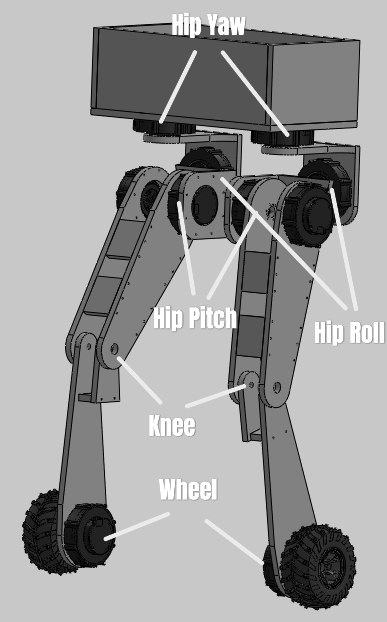
\includegraphics[width=0.50\linewidth]{figures/annotated_robot_joints_bw.png}
    \caption{Robot joint layout with world frame (right-handed, $Z$ up). Wheel axles lie along world $X$, so the rolling (and therefore sagittal) direction is world $Y$ and world $X$ is the lateral (track) axis. Each leg: hip roll (HR), hip yaw (HY), hip pitch (HP), knee (KN), wheel (WH).}
    \label{fig:robot}
\end{figure}

% ============================================================
\section{ACC Formulation}
% ============================================================

\subsection{Two-Channel Torque Assembly}
\label{sec:overview}

ACC assembles a PD balance core, a proximity-gated anchor integral and posture
regulation into two torque channels, wheel torque
($\boldsymbol{\tau}_w\in\mathbb{R}^2$) and leg-joint torque
($\boldsymbol{\tau}_q\in\mathbb{R}^8$), with flight and terrain as independent extensions (Fig.~\ref{fig:acc_arch}):

\begin{equation}
\begin{aligned}
\boldsymbol{\tau}_w &= (1-g_{\text{flight}})\!\big[\boldsymbol{\tau}_{\text{balance}} + g_{\text{anchor}}\boldsymbol{\tau}_{\text{anchor}}\big] + g_{\text{flight}}\boldsymbol{\tau}_{\text{flight}},\\
\boldsymbol{\tau}_q &= \boldsymbol{\tau}_{\text{posture}}\big(h^{\text{cmd},L},\,h^{\text{cmd},R}\big) + \boldsymbol{\tau}_{\text{lat}} + \boldsymbol{\tau}_{\text{yaw}}.
\end{aligned}
\label{eq:two_channel}
\end{equation}

Neither gate is a summand. At $g_{\text{flight}}{=}1$ the flight term
\emph{replaces} the wheel torque, since the balance core regulates against a ground that is no longer there, and the convex blend is what makes the replacement
continuous. Per-leg ground adaptation likewise enters as a \emph{reference}
split: the posture regulator always takes two height commands, coincident on
level ground, while $g_{\text{terrain}}$ itself acts in the wheel channel.

Every gate $g_*$ except the flight gate is a \emph{smoothstep} function of a
physical condition (proximity, quietness, attitude, terrain disparity) rather
than a discrete switch:

\begin{equation}
\operatorname{ss}(x;a,b) = 3t^2 - 2t^3,
\qquad t = \operatorname{clip}\!\left(\frac{x-a}{b-a},\,0,\,1\right).
\label{eq:smoothstep}
\end{equation}

Equation~\eqref{eq:smoothstep} is the standard Hermite blend, $C^1$ in $x$ with
zero derivative at both knees. Continuity matters concretely: a hard threshold
injects a torque step equal to the full gated component, which at \SI{100}{Hz}
under a \SI{400}{Nm/s} rate limit reaches the plant as an unmodelled impulse.
The one exception is $g_{\text{flight}}$, and only on the way in: contact loss is
a binary physical event, so engagement is a latched load-based hysteresis with
asymmetric timers. Its handback is not discrete: after release the gate ramps linearly $1\to0$ over \SI{150}{ms}, since an instant handback at large pitch
returns full wheel authority (${\sim}\SI{19}{Nm}$) to a marginally loaded wheel
and re-launches the robot.

Wheel torques control sagittal balance; lateral and yaw regulation actuate in
the leg-joint channel through the antisymmetric hip-roll and hip-yaw pairs
(Eq.~\eqref{eq:lat_yaw}), the wheels carrying no roll or yaw differential. On
level ground the channels are then coupled only through the plant, the terrain
gate being identically zero. Across a step it opens, softening $k_{\text{pos}}$, raising the position-torque cap, adding a pitch-rate
feedforward and symmetrising the per-wheel damping, but that coupling vanishes
continuously with the height split, so flight recovery and terrain adaptation
are still added without retuning the anchor. Unlike the industrial override architectures of
\S\ref{sec:related_dist}, which select \emph{among parallel controllers} on
process-variable limits, ACC gates \emph{components within a single torque
assembly} on physical quantities of three kinds (spatial, temporal and safety-interlock), each chosen because a specific measured failure mode of this
platform is expressible in it.

\begin{figure}[htbp]
    \centering
    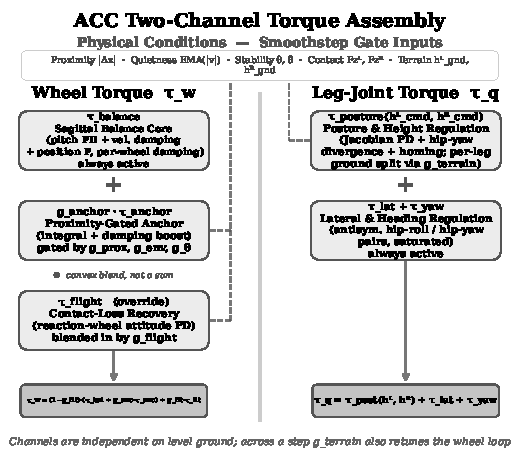
\includegraphics[width=0.92\linewidth]{figures/acc_architecture_bw.pdf}
    \caption{ACC two-channel torque assembly. Physical conditions gate each component via continuous smoothstep functions (dashed). The latched flight gate \emph{overrides} the wheel channel rather than adding to it, and per-leg ground adaptation enters as a split pair of height references, not an added torque.}
    \label{fig:acc_arch}
\end{figure}

\subsection{Sagittal Balance Core ($\boldsymbol{\tau}_{\text{balance}}$)}
\label{sec:balance_core}

The sagittal balance component is always active and acts entirely in the
wheel-torque channel:

\begin{equation}
\boldsymbol{\tau}_{\text{balance}} =
\begin{bmatrix}
\tau_{\text{com}} + \tau_{w}^{L} \\
\tau_{\text{com}} + \tau_{w}^{R}
\end{bmatrix},
\;
\begin{aligned}
\tau_{\text{com}} &= \tau_{\text{pitch}} + \tau_{\text{damping}} + \tau_{\text{pos}},\\
\tau_{w}^{i} &= -k_{w}\big(\omega^{i} - \omega^{\text{cmd}}\big),
\end{aligned}
\label{eq:balance}
\end{equation}

with $\tau_{\text{com}}$ identical on both wheels and the per-wheel damping
$\tau_{w}^{i}$ ($i\in\{L,R\}$) the only term that differs between them,

while lateral and yaw regulation, which read torso state alongside the balance
core, actuate antisymmetrically on the hip-roll pair
$(\mathrm{HR}^L,\mathrm{HR}^R)$ and the hip-yaw pair
$(\mathrm{HY}^L,\mathrm{HY}^R)$ of the leg-joint channel:

\begin{align}
\tau_{\text{pitch}} &= k_p\cdot\theta + k_d\cdot\dot{\theta},\\
\tau_{\text{damping}} &= -\big(s_v k_{\text{vel}} + k_{v2}\big)\cdot v_{\text{sag}},\\
\tau_{\text{pos}} &= -k_{\text{pos}}\cdot\operatorname{clip}(\Delta x,\,\pm\SI{0.10}{m}),\\
\boldsymbol{\tau}_{\text{lat}} &= \big[{+}1,\,{-}1\big]^{\!\top}
\big(k_{p,\text{roll}}\phi + k_{d,\text{roll}}\dot{\phi}\big),
\label{eq:lat_yaw}\\
\boldsymbol{\tau}_{\text{yaw}} &= \big[{-}1,\,{+}1\big]^{\!\top}
\big(k_{p,\text{yaw}}e_\psi - k_{d,\text{yaw}}\omega_z\big),
\end{align}

the last two saturated at their own moment limits, with $s_v$ the scheduled
damping scale, $k_{v2}$ a fixed unscheduled damping offset, $\theta$ torso pitch,
$v_{\text{sag}}$ the sagittal body velocity, $\Delta x$ the sagittal position
error from the latched home position, $\phi$ the roll angle, $e_\psi$ the yaw
error and $\omega_z$ the yaw rate. The lateral axis is thus closed by the legs,
and the fixed sign pattern of these two pairs is the mechanism behind the
chirality of the push envelope.

The P position term ($k_{\text{pos}}$, clipped to $\pm\SI{0.10}{m}$, saturating
at $\pm\SI{4}{Nm}$) keeps the robot within $\pm$\SIrange{4}{6}{cm} of home but
leaves a \SI{1.3}{Nm} equilibrium bias sustaining a perpetual limit cycle, which
motivates the anchor integral. Saturation-triggered anti-windup does not address
it, the critical failure being \emph{state-dependent}: during a push, position
error grows to \SIrange{10}{30}{cm} while the wheels remain within their
\SI{20}{rad/s} range, so a saturation trigger never fires and ACC uses spatial
confinement instead. Pitch stiffness is fixed at $k_p{=}50$; a scheduled variant
softening it to \num{35} during pushes was tested and rejected (S0 vs.\ S1,
Table~\ref{tab:push_ablation}).

\subsection{Proximity-Gated Anchor ($g_{\text{anchor}}\boldsymbol{\tau}_{\text{anchor}}$)}
\label{sec:anchor}

The anchor mechanism is the core contribution. It adds three terms to the
wheel-torque channel that are active only when the robot is near home \emph{and}
genuinely at rest:

\begin{equation}
\begin{split}
\boldsymbol{\tau}_{\text{anchor}} = {}
& K_i\!\int\! g_{\text{prox}}\cdot g_{\text{env}}\cdot(-\Delta x)\,dt\\
& + g_{\text{boost}}\cdot K_{\text{boost}}\cdot(-v_{\text{sag}})\\
& + \bigl(k_{d,h}g_h + k_{d,a}g_{\text{prox}}\bigr)g_{\dot{\theta}}\cdot(-\dot{\theta}),
\end{split}
\label{eq:anchor}
\end{equation}

where the gates are continuous smoothstep functions equal to $1$ when the robot
is ``at home and quiet'' and transitioning smoothly to $0$ otherwise:

\begin{align}
g_{\text{prox}}(\Delta x) &= 1 - \operatorname{ss}\bigl(|\Delta x|;\;\SI{0.05}{m},\,\SI{0.15}{m}\bigr),
\label{eq:g_prox}\\[2pt]
g_{\text{env}}(v_{\text{sag}}) &= 1 - \operatorname{ss}\bigl(\mathrm{EMA}(|v_{\text{sag}}|);\;\SI{0.25}{m/s},\,\SI{0.50}{m/s}\bigr),
\label{eq:g_env}\\[2pt]
g_\theta(\theta,\dot{\theta}) &= \bigl[1 - \operatorname{ss}(|\theta|;\,\SI{2}{\degree},\,\SI{12}{\degree})\bigr] \nonumber\\
&\quad\times \bigl[1 - \operatorname{ss}(|\dot{\theta}|;\,\SI{2}{\degree/s},\,\SI{15}{\degree/s})\bigr],
\label{eq:g_theta}\\[2pt]
g_h(\Delta h) &= 1 - \operatorname{ss}\bigl(|\Delta h|;\;\SI{0.05}{mm},\,\SI{0.30}{mm}\bigr),
\label{eq:g_h}\\[2pt]
g_{\dot{\theta}}(\dot{\theta}) &= \operatorname{ss}\bigl(|\dot{\theta}|;\,\SI{2}{\degree/s},\,\SI{15}{\degree/s}\bigr),
\label{eq:g_thetadot}\\[2pt]
g_{\text{boost}} &= g_{\text{prox}}\cdot g_{\text{env}}\cdot g_\theta.
\label{eq:g_boost}
\end{align}

Each gate is dimensionless, monotone and $C^1$, and three physically distinct
conditions must hold simultaneously for the anchor to integrate: spatially near
home ($g_{\text{prox}}$), temporally quiet ($g_{\text{env}}$) and attitudinally
settled ($g_\theta$). The pitch gate closes when either pitch or pitch rate
leaves its band, preventing the damping boost from fighting a gentle sustained
push that does not trigger the velocity envelope.

\textbf{Asymmetric envelope follower.} Reliable quiet-stance detection rests on
an asymmetric exponentially-weighted moving average (EMA) of $|v_{\text{sag}}|$:
\begin{equation}
\text{EMA}_t = \begin{cases}
\alpha_a|v_t| + (1{-}\alpha_a)\text{EMA}_{t-1}, & |v_t| > \text{EMA}_{t-1},\\
\alpha_r|v_t| + (1{-}\alpha_r)\text{EMA}_{t-1}, & \text{else},
\end{cases}
\label{eq:asym_ema}
\end{equation}
with time constants $\tau_{\text{attack}}{\approx}\SI{23}{ms}$ and
$\tau_{\text{release}}{\approx}\SI{1.5}{s}$ as the primary specification, the
discrete coefficients following as $\alpha_a{=}1{-}e^{-\Delta t/\tau_{a}}
\approx 0.35$ and $\alpha_r \approx 0.007$ at \SI{100}{Hz}. The asymmetry is
essential: a symmetric EMA is \emph{bistable}: post-push oscillation holds it
in a middle band where the gate is half-open and the boost cannot collapse the
cycle, as the symmetric-EMA ablation of \S\ref{sec:results} confirms, whereas the fast-attack/slow-release envelope rises to $1$ only when oscillation truly
decays and drops to $0$ within ${\sim}\SI{25}{ms}$ of a disturbance. The
mechanism is a peak-hold envelope detector; ACC's contribution is coupling it to
a spatial proximity gate for integral conditioning. Since $\text{EMA}_0{=}0$
biases $g_{\text{env}}{\approx}1$ for ${\sim}\SI{7.5}{s}$ at startup, all
measurements discard a \SIrange{3}{5}{s} settle interval.

\subsection{Posture and Yaw Stability ($\boldsymbol{\tau}_{\text{posture}}$)}
\label{sec:posture}

Posture regulation uses Jacobian-based PD gains scheduled across \num{23}
heights:

\begin{equation}
\begin{split}
\boldsymbol{\tau}_{\text{posture}} =\;&
\boldsymbol{\tau}_{\text{PD}}^{\text{jac}}(q,\dot{q},h^{\text{cmd}})
+ \boldsymbol{\tau}_{\text{div}}(q_{\text{hy}}^L,q_{\text{hy}}^R)\\
&+ g_{\text{settled}}\,\boldsymbol{\tau}_{\text{homing}}(q-q_{\text{ref}}),
\end{split}
\label{eq:posture}
\end{equation}

where $\boldsymbol{\tau}_{\text{div}}$ damps hip-yaw divergence and
$\boldsymbol{\tau}_{\text{homing}}$ restores nominal posture when upright and
settled. Yaw return uses wheel-differential torque.

\subsection{Extensions: Contact Loss and Per-Leg Terrain}
\label{sec:extensions}

Two extensions attach to the same assembly without re-tuning the anchor, and
both vanish identically in nominal standing. \emph{Contact-loss recovery}
($g_{\text{flight}}$): when both wheels report $F_z < 0.5mg$ for two consecutive
steps, ACC substitutes a flight attitude controller that uses the wheels as
reaction flywheels, $\boldsymbol{\tau}_{\text{flight}} =
\operatorname{clip}(2.0\theta + 0.5\dot{\theta} -
0.02\omega_{\text{wheel}},\,\pm\SI{2}{Nm})$, with a five-step loaded-release
hysteresis so balance torque cannot re-engage mid-bounce. \emph{Per-leg ground
adaptation} ($g_{\text{terrain}}$): a wheel resting at a different ground height
would otherwise force the torso to roll by the step angle, so ACC maintains an
independent ground estimate per leg from the wheel contact-point height (exact at any body tilt for a rigid wheel), updated only while that wheel carries at
least $0.2mg$, and absorbs the disparity by a \emph{kinematic} leg-length split
plus a closed-loop levelling integrator trimming the residual by the measured
roll. Both are specified in full, with their ablation matrices, in the extended
version.

\subsection{Complete Numerical Parameter Set}
\label{sec:parameters}

\begin{sloppypar}
The core gains are $k_p{=}\SI{50}{Nm/rad}$, $k_d{=}\SI{10}{Nm/(rad/s)}$,
$k_{\text{pos}}{=}\SI{40}{Nm/m}$ (clipped at $\pm\SI{4}{Nm}$),
$k_{\text{vel}}{=}\SI{15}{Nm/(m/s)}$ at damping scale $s_v{=}\num{1.5}$ plus a
fixed $k_{v2}{=}\SI{5}{Nm/(m/s)}$, $k_w{=}\SI{0.5}{Nm/(rad/s)}$,
$k_{\text{roll}}{=}\SI{55}{Nm/rad}$, $k_{\text{yaw}}{=}\SI{1.0}{Nm/rad}$; the
anchor uses $K_i{=}\SI{4.0}{Nm/(m.s)}$ capped at \SI{2}{Nm} with a
$5\times10^{-3}$ per-step leak, boost scale \num{5.0}, gated pitch-rate gains
$k_{d,h}{=}3.0$ and $k_{d,a}{=}\SI{7.0}{Nm/(rad/s)}$ over a $g_h$ band of
\SIrange{0.05}{0.30}{mm}, $g_{\text{prox}}$ band
\SIrange{0.05}{0.15}{m}, $g_{\text{env}}$ band \SIrange{0.25}{0.50}{m/s},
$g_{\text{stab}}$ bands \SIrange{2}{12}{\degree} and
\SIrange{2}{15}{\degree\per\second}; flight uses P/D $=2.0/0.5$ with
\SI{0.02}{Nm/(rad/s)} wheel damping and $2/5$-step engage/release at
$F_z{=}0.5mg$ ($0.2mg$ for terrain). The full set (50+ gains) is in the
supplementary material.
\end{sloppypar}

% ============================================================
\section{Experimental Validation}
\label{sec:results}
% ============================================================

ACC and all six classical baselines are evaluated at \SI{500}{Hz} physics /
\SI{100}{Hz} control under a \SI{400}{Nm/s} per-joint torque rate limit, so the
headline comparison is rate-matched by construction; the PPO reference is
reported at the \SI{50}{Hz} rate its policy was trained at. Each classical
baseline was additionally measured at its own \SI{50}{Hz} design rate: the fall
rate is \SI{100}{\percent} in all twelve cells and five of the six survive
\emph{longer} at \SI{50}{Hz}, so reporting them at \SI{100}{Hz} is the
rate-matched choice and the harsher of the two for them. Seeds are deterministic:
$20260727{+}\text{trial\_id}$ for idle standing,
$20260728{\times}100{+}\text{rep}$ for the push ablation, and $\{0,42,123\}$ for
the classical baselines.

\subsection{Anchored Standing}
\label{sec:standing}

\subsubsection{Metrics and axis convention}

``Standing precision'' names two quantities that are not interchangeable. With
$\mathbf{p}(t)\in\mathbb{R}^2$ the horizontal base position over a window of
length $T$, $\mathbf{p}_0$ the commanded home and $\bar{\mathbf{p}}$ the trial
mean,
\begin{align}
A &= \Bigl(\tfrac{1}{T}\textstyle\int_0^T \lVert\mathbf{p}(t)-\mathbf{p}_0\rVert^2\,dt\Bigr)^{1/2},
\label{eq:accuracy}\\
R &= \Bigl(\tfrac{1}{T}\textstyle\int_0^T \lVert\mathbf{p}(t)-\bar{\mathbf{p}}\rVert^2\,dt\Bigr)^{1/2}
\label{eq:repeatability}
\end{align}
define the \emph{accuracy} $A$, which retains any DC parking offset, and the
\emph{repeatability} $R$, which removes it; the two differ by more than an order
of magnitude here, so both are reported for every configuration. Each is
resolved along the sagittal axis, the lateral axis and the full plane, the two
horizontal axes being actuated by different means: the \textbf{sagittal} axis is
world $y$, the rolling direction and the only one on which wheel torque produces
ground force, while the \textbf{lateral} axis is world $x$, held passively by the
wheel contacts and the roll restoring moment of the track width. A dynamic check
confirms the assignment (\texttt{scripts/verify\_body\_axes.py}): a \SI{90}{N}
impulse along $y$ is absorbed at a peak wheel speed of \SI{52}{rad/s} leaving
\SI{4.8}{mm} of residual offset, whereas the same impulse along $x$ leaves a
permanent \SI{23.2}{mm} offset. The anchor integral and the gated damping boost
both live in the wheel-torque channel, so both act sagittally only.

\subsubsection{Protocol}

Every row of Table~\ref{tab:standing} is measured under one protocol:
\SI{25}{s} from the nominal standing pose with randomised initial conditions
($\sigma{=}\SI{0.005}{rad}$ per joint, clipped to limits; $\sigma{=}\SI{1}{mm}$
on root height), with $A$, $R$ taken relative to each trial's own $t{=}0$ pose
after a settle covering the EMA$_0{=}0$ transient to within \SI{1}{\percent}. A
trial is a fall if $|\theta|{>}\SI{46}{\degree}$ or root height
${<}\SI{0.15}{m}$; confidence intervals are Student-$t$. This measures the
ability to \emph{stay} put; coming back is measured in \S\ref{sec:push}.

\begin{table*}[tp]
\centering
\caption{Idle standing precision across the full ablation ladder. All rows
measured under the single protocol of \S\ref{sec:standing}; values are
mean${\pm}$SD over $N{=}10$ trials.}
\label{tab:standing}
\footnotesize
\setlength{\tabcolsep}{4pt}
\begin{tabular}{@{}ll S[table-format=2.3(4)] S[table-format=2.3(3)] S[table-format=2.3(4)] S[table-format=-2.1] c@{}}
\toprule
& \multirow{2}{*}{Configuration}
& {$R_{\text{sag}}$ (mm)} & {$R_{xy}$ (mm)} & {$R_{\text{lat}}$ (mm)} & {$\bar{s}$ (mm)} & Survival \\
& & {sagittal rep.} & {planar rep.} & {lateral rep.} & {sag.\ offset} & \\
\midrule
\multicolumn{7}{@{}l}{\textbf{Additive ladder (bottom-up)}}\\
L0   & P-only (PD, no position, no integral) & 17.461(258) & 17.845(279) & 3.675(246) & -44.8 & 10/10 \\
L1   & $+$ position homing ($\pm\SI{0.10}{m}$) & 20.397(17) & 20.414(19) & 0.834(66) & -30.4 & 10/10 \\
L2   & $+$ ungated integral $K_i$ & 25.026(39) & 25.056(43) & 1.212(110) & -27.5 & 10/10 \\
L2.5 & $+$ proximity gate only (no envelope, no boost) & 25.198(17) & 25.227(20) & 1.205(99) & -27.6 & 10/10 \\
\midrule
\multicolumn{7}{@{}l}{\textbf{Proposed controller}}\\
L3/S1 & \textbf{ACC} (full anchor, fixed $k_p{=}50$) & \bfseries 0.294(15) & \bfseries 0.788(69) & \bfseries 0.730(73) & \bfseries -27.0 & \textbf{10/10} \\
\midrule
\multicolumn{7}{@{}l}{\textbf{Subtractive ablation (top-down from ACC)}}\\
S2 & $-$ gated damping boost & 4.772(69) & 4.824(67) & 0.703(69) & -26.8 & 10/10 \\
S3 & $-$ asymmetric envelope (symmetric EMA) & 0.294(15) & 0.788(69) & 0.730(73) & -27.0 & 10/10 \\
S4 & $-$ proximity gate (integral always on) & 0.294(15) & 0.788(69) & 0.730(73) & -27.0 & 10/10 \\
S5 & $-$ pitch safety gate $g_\theta$ & {---} & {---} & {---} & {---} & \textbf{0/10} \\
\midrule
\multicolumn{7}{@{}l}{\textbf{Single-mechanism isolation (ACC with one term disabled)}}\\
M1 & $K_i{=}0$ (anchor integral removed, gates intact) & 0.089(35) & 0.733(72) & 0.727(71) & -31.2 & 10/10 \\
M2 & damping terms reverted to their L2 values & 25.198(17) & 25.227(20) & 1.205(99) & -27.6 & 10/10 \\
M3 & $K_i{=}0$ \emph{and} boost $=0$ & 3.973(130) & 4.037(128) & 0.710(69) & -31.1 & 10/10 \\
\bottomrule
\end{tabular}
\vspace{2pt}\tabnote\noindent
\SI{100}{Hz} control, \SI{20}{s} window after a \SI{5}{s} settle, clean sensors,
\SI{0}{ms} delay. $R$ = repeatability (Eq.~\eqref{eq:repeatability}); $\bar{s}$
= mean signed sagittal parking offset; accuracy on an axis is that offset and
the repeatability in quadrature, so the $A$ columns are omitted (the identity
holds to \SI{0.003}{mm} on every surviving row). Sagittal is world $y$, lateral
world $x$; the anchor integral and the damping boost act sagittally only, so
$R_{\text{sag}}$ and $\bar{s}$ discriminate between configurations while
$R_{\text{lat}}$ measures a passively held axis. Produced by
\path{scripts/collect_idle_ladder.py}.
\end{table*}

\subsubsection{Result}

ACC holds \textbf{sub-millimetre sagittal repeatability},
$R_{\text{sag}}=0.294{\pm}\SI{0.015}{mm}$ (95\%\,CI $[0.283,0.305]$\,mm) across
ten randomised trials with no falls. This is the figure of merit for the platform,
sagittal being the actuated inverted-pendulum axis. Precision is assessed from
the relative spread \emph{between} configurations under an identical protocol
rather than against a simulator noise floor: removing a single mechanism (S2)
moves $R_{\text{sag}}$ sixteenfold with non-overlapping SDs. Against the P-only
baseline L0, which sustains a \SI{69.7}{mm} peak-to-peak sagittal limit cycle,
the like-for-like improvements are \textbf{59.4}$\times$ sagittal,
\textbf{22.6}$\times$ planar and \textbf{5.0}$\times$ lateral, largest on the hard axis and smallest on the easy one, the correct signature for a wheel-torque
controller, since every term ACC adds beyond L0 produces ground force along the
rolling direction and none can produce lateral force at all.

Accuracy and repeatability are distinct on this axis. ACC parks at
$\bar{s}={-}\SI{27.0}{mm}$ from commanded home and holds that standoff to
\SI{0.009}{mm} SD across trials, so planar accuracy is
$A_{xy}=\SI{26.994}{mm}$, a $1.8{\times}$ improvement over L0 against the
$59{\times}$ gain in repeatability. Its magnitude is fully accounted for:
instrumenting the sagittal torque balance predicts the offset in closed form
from a \emph{leaky} anchor integral whose ${\sim}\SI{2}{s}$ forgetting horizon
fixes its DC gain at the finite $k_{I,\text{dc}}{=}\SI{7.96}{Nm/m}$, so a constant load leaves a finite error by construction, and a \SI{1.44}{\degree} error in the feedforward pitch reference, giving \SI{24.88}{mm} against
\SI{24.99}{mm} measured and holding across a $40{\times}$ gain sweep and a
five-point height sweep to within \SI{0.92}{\percent}. The leak also buys the
steadiness: a $10{\times}$ smaller $\lambda$ cuts the offset to \SI{-16.31}{mm}
but degrades window jitter twelvefold, so Table~\ref{tab:standing} publishes a
chosen point on that trade-off.

\subsubsection{The measurement window is a protocol choice, not a stability
horizon}
\label{sec:longhorizon}

Every row of Table~\ref{tab:standing} is measured over \SI{20}{s}, and that
standard cuts both ways. Re-running the ACC row with identical seeds, initial conditions, profile and metrics, and only the window lengthened, reproduces
$0.294{\pm}\SI{0.015}{mm}$ at \SI{20}{s} and then \emph{improves} on it, to
$0.089{\pm}\SI{0.005}{mm}$ at \SI{300}{s} (10/10, drift $+\SI{0.0149}{mm/min}$)
and $0.037{\pm}\SI{0.002}{mm}$ at \SI{1800}{s} (4/4, $+\SI{0.0004}{mm/min}$): the
\SI{20}{s} figure is the conservative one, that window still containing the tail
of the settle. The settle terminates in a fixed point, not a slow mode: after ${\approx}\SI{35}{s}$ the sagittal coordinate is constant to
\SI{2e-6}{mm} per \SI{30}{s} block for the remaining twenty-nine minutes at a
\SI{-26.763}{mm} parking offset, the only motion left a \SI{0.14}{mm/hour}
lateral creep on the passively held axis. The full-state LQR of
Section~\ref{sec:full_state_lqr}, by contrast, accumulates
\SIrange{0.43}{0.63}{m} of planar drift and falls, having no term that
references position to a latched home; ACC has two, the clipped proportional
$\tau_{\text{pos}}$ of Eq.~\eqref{eq:balance} and the anchor integral on
$-\Delta x$ of Eq.~\eqref{eq:anchor}.\footnote{Seeds
$20260727{+}i$, \SI{5}{s} settle, clean sensors, \SI{0}{ms} delay, as in
Table~\ref{tab:standing}; produced by \path{scripts/idle_longhorizon.py}.}

\subsubsection{Which mechanism produces the precision}
\label{sec:idle_mechanism}

The lower blocks of Table~\ref{tab:standing} isolate the contributions; three of
the four findings contradict the attribution the gate structure invites.
\emph{(i) Idle steadiness comes from the damping ladder; the integral buys
accuracy instead.} M1 disables the anchor integral ($K_i{=}0$) with every gate in
place, and its repeatability is slightly better than ACC's while its accuracy is
worse by \SI{4.2}{mm}; M2 keeps the integral and every gate but reverts the two
velocity-damping coefficients to their L2 values, reproducing the L2/L2.5 limit
cycle exactly. Steadiness is therefore attributable to the damping terms, in two
stages: raising the velocity-damping scale takes $R_{\text{sag}}$ to
\SI{3.97}{mm} (M3), the gated boost the rest of the way, a combined factor of \num{86}. \emph{(ii) The damping boost acts sagittally, as it must.} S2 degrades
sagittal repeatability sixteenfold while leaving lateral repeatability
statistically unchanged (overlapping CIs), the only outcome consistent with a
boost inside the wheel-torque channel.

\emph{(iii) The proximity gate and the asymmetric envelope are inert during
quiet stance.} Ablating either (S4, S3) is \emph{bit-identical} to ACC on every idle metric, because the base never leaves the \SI{5}{cm} inner band and the velocity
envelope never rises into the attack branch, so both are evaluated only in
Table~\ref{tab:push_ablation}. \emph{(iv) The pitch safety gate is required even
to stand.} S5 falls \num{10}/\num{10} during quiet stance with no push applied:
removing $g_\theta$ lets the damping boost act on the pitch state at large
excursions, and the resulting positive feedback diverges from the
${\pm}\SI{0.005}{rad}$ initial perturbation alone.

\subsection{Omnidirectional Push Recovery}
\label{sec:push}

Push recovery is evaluated by polar sweep: \SIrange{10}{160}{N} impulses of
\num{7} control steps applied at the torso in \num{8} world-frame directions
($\theta{=}\pm\SI{90}{\degree}$ sagittal,
$\theta{=}\SI{0}{\degree}/\SI{180}{\degree}$ lateral), each threshold located by
binary search to \SI{5}{N}, survival being torso pitch $<\SI{46}{\degree}$ for
\SI{17}{s} post-push; $F_{\min}$ is the maximum magnitude survived in
\emph{every} direction, $F_{\text{med}}$ the median.

\emph{The envelope is anisotropic by construction.} Per-bearing means span
\SIrange{82.1}{144.1}{N}: the two lateral bearings average \SI{98.0}{N} against
\SI{130.0}{N} for the two sagittal ones, the weakest being the oblique
\SI{45}{\degree} (\SI{82.1}{N}, \SI{24}{\percent} below $F_{\text{med}}$). This
follows from the morphology, not the tuning: the wheels drive the contact patch
back under the CoM sagittally but produce no lateral ground force, so raising the
lateral bearing requires a centralised lateral task (\S\ref{sec:wbc}), not a gain
change.

\emph{The envelope is also chiral, and the chirality is in the controller.}
Superposed on the anisotropy is a left--right asymmetry: \SI{135}{\degree}
survives \SI{40.7}{N} more than $-\SI{135}{\degree}$. The plant cannot produce it: mirroring the model about the sagittal plane reproduces its mass, inertia
and geometry to \SI{0.05}{mm} and \num{1e-7}, and a harmonic fit localises the
violation in the mirror-forbidden term ($b_2{=}\SI{-17.3}{N}$ against
$b_1{=}\SI{0.3}{N}$). Under a mirrored state the commanded torque maps to its own
mirror image on hip-pitch, knee and wheel and fails only on hip-roll and hip-yaw,
both assembled antisymmetrically; mirroring those two channels flips $b_2$ to
\SI{+15.6}{N} at unchanged magnitude, a sham mirror leaving it at \SI{-15.7}{N}.
The correction is reported but not adopted, redistributing the envelope without
enlarging it ($F_{\min}$ \SI{82.5}{}${\rightarrow}\SI{79.7}{N}$). Later protocols
push along world $+x$, a lateral and below-median bearing (\SI{95.5}{N}), so they
are conservative probes.

\begin{table}[htbp]
\centering
\footnotesize
\caption{Factorial ablation of ACC components: push-recovery and ringdown metrics. Clean sensors, all rows $N{=}30$, mean${\pm}$std.}
\label{tab:push_ablation}
\setlength{\tabcolsep}{3pt}\begin{tabular}{@{}c>{\raggedright\arraybackslash}p{2.85cm}rr>{\raggedright\arraybackslash}p{1.35cm}@{}}
\toprule
& Configuration & $F_{\min}$ (N) & $F_{\text{med}}$ (N) & Ringdown \\
\midrule
\multicolumn{5}{@{}l}{\textbf{Additive (bottom-up)}} \\
\midrule
L0 & P-only (PD, no pos., no I)  & 70.0${\pm}$1.3 & 122.8${\pm}$3.3 & never \\
L1 & $+$\,Pos.\ homing ($\pm$\SI{0.10}{m}) & 75.0${\pm}$1.1 & 130.5${\pm}$1.9 & never \\
L2 & $+$\,Integral $K_i$ (no gate) & 74.9${\pm}$0.9 & 131.5${\pm}$1.4 & --- \\
L2.5 & $+$\,Prox.\ gate only (no EMA, no boost) & 74.9${\pm}$0.9 & 131.4${\pm}$2.0 & --- \\
L3 & $+$\,Full anchor (gate, EMA, boost) & \bfseries 82.1${\pm}$2.7 & 108.4${\pm}$6.6 & \textbf{\SI{9.0}{s}} \\
\midrule
\multicolumn{5}{@{}l}{\textbf{Subtractive (top-down from ACC)}} \\
\midrule
S0 & ACC $+$ scheduled $k_p$ (rejected)  & 80.7${\pm}$2.8 & 110.2${\pm}$6.2 & \SI{9.0}{s} \\
S1 & \textbf{ACC} (canonical, fixed $k_p{=}50$) & \bfseries 82.1${\pm}$2.7 & 108.4${\pm}$6.6 & \textbf{\SI{9.0}{s}} \\
S2 & $-$Damping boost           & 81.2${\pm}$1.0 & 115.9${\pm}$6.2 & never \\
S3 & $-$Asym.\ EMA (sym.\ EMA)  & 81.5${\pm}$2.6 & 106.1${\pm}$6.2 & never \\
S4 & $-$Prox.\ gate (global I)  & 80.7${\pm}$2.8 & 110.2${\pm}$6.2 & windup \\
S5 & $-$Pitch gate $g_\theta$   & ${<}10$ & ${<}10$ & never \\
\bottomrule
\end{tabular}
\vspace{2pt}\tabnote\noindent
$F_{\min}$ and $F_{\text{med}}$ are the minimum and median survivable push over
\num{8} bearings, each located by binary search to \SI{5}{N} tolerance; idle
metrics for the same configurations are in Table~\ref{tab:standing}. The S5
entries are left-censored: in \num{231} of \num{240} trials the bisection found
no survivable magnitude in $[\SI{10}{N},\SI{160}{N}]$ and the nine exceptions
reach at most \SI{46.3}{N}, so both are upper bounds. Welch's unpaired two-sided
$t$-test ($N{=}30$ per group, Bonferroni-adjusted $\alpha{=}0.0056$, \num{9}
comparisons): L0$\rightarrow$L1 $+\SI{5.1}{N}$, $p{=}\num{2e-23}$, $d{=}4.3$;
L1$\rightarrow$L2 $p{=}0.69$; L2$\rightarrow$L2.5 $p{=}0.86$;
L2.5$\rightarrow$L3 $+\SI{7.2}{N}$, $p{=}\num{1e-15}$, $d{=}3.6$. No subtractive
row differs significantly from ACC except S5 ($p{=}\num{2e-44}$), and those four
nulls are bounded rather than underpowered ($|d|{\le}0.49$, ${<}\SI{1.4}{N}$ on
$F_{\min}$). The 95\%\,CI half-width is ${\approx}0.37{\times}$std, so the push
rows resolve ${\approx}\SI{1}{N}$. Each trial starts from a freshly constructed
controller context. Produced by \path{scripts/replicate_ablation_n30.py}.
\end{table}

Table~\ref{tab:push_ablation} reports the factorial ablation. Additively, only
homing (L1) and the full anchor (L3) add significant margin; the global integral
and the proximity gate add nothing to push \emph{margin} on their own (the gate prevents windup, it does not enlarge the capture basin) and the full anchor is
the only rung that settles. Subtractively the ablation is flat: at $N{=}30$ every
single-mechanism removal except the pitch gate leaves $F_{\min}$ within
\SI{1.4}{N} of ACC ($|d|{\le}0.49$), so the capture basin is set by the anchor as
a whole, not by any one of its four gates, including gain scheduling (S0) and
the damping boost, which dominates idle precision yet leaves push margin
indistinguishable from ACC's (S2). Removing the pitch gate (S5) leaves the robot
unable to survive even the search floor. Ringdown decays within \SI{9}{s} under
ACC, whereas P-only oscillates indefinitely on the \SI{1.3}{Nm} equilibrium bias;
symmetric EMA shows the bistable failure the asymmetry prevents, and the ungated
integral winds up during the push and never settles.

\subsection{Flight Recovery and Terrain Adaptation}
\label{sec:flight_terrain_results}

At $N{=}10$ randomised-IC trials, ACC settles \num{10}/\num{10} from every drop and ledge tested (peak $|\theta|$ of $24.0{\pm}\SI{1.2}{\degree}$ on a
\SI{100}{cm} drop and $27.1{\pm}\SI{2.0}{\degree}$ on a \SI{50}{cm} ledge) and traverses \num{10}/\num{10} at every curb height to \SI{20}{cm}
(\SI{0.15}{m/s}) at a straddle roll of $2.4{\pm}\SI{0.1}{\degree}$ to
$3.9{\pm}\SI{0.1}{\degree}$. Replacing the per-leg split with a symmetric
posture falls at \emph{every} curb height.


\subsection{Comparison with Classical Baselines and a Preliminary RL Reference}
\label{sec:baselines}

No balance controller has been published for this morphology, so no established
classical design exists for this plant to compare against. What can be measured
instead is \emph{transfer}: how far the reduced-order controllers the
wheeled-biped literature does publish carry when applied here. Read the rows
below as a transfer result rather than as a ranking of ACC against optimal
control; the row that tests the linear-design family on its own terms is the
full-state controller of \S\ref{sec:full_state_lqr}. Six classical baselines are
evaluated under identical environment setups: four derived from the
4-state TWIP model~\citep{grasser2002joe} (LQR with decoupled roll/yaw PD
through a PID servo layer of ${\sim}\SI{0.25}{s}$ lag; the same plus a
pitch-error integral with conditional anti-windup; a direct-torque variant
re-optimised for the zero-lag plant; and PI$+$AW, adding a conditional
forward-position integral) and two 6-state coupled variants adding the roll
states $(\phi,\dot\phi)$, one through the servo and one commanding torque
directly, all weights following Bryson's rule~\citep{bryson1975optimal}. A model-free PPO run
(\num{5.4}M steps, single seed, no domain randomisation or hyperparameter
search) is reported alongside as a difficulty probe, not a tuned RL baseline
(Limitation~4).

\begin{table}[htbp]
\centering
\footnotesize
\caption{Classical baselines and the preliminary PPO reference vs.\ ACC, clean sensors. All rows at \SI{100}{Hz} control except the PPO reference, which is reported at the \SI{50}{Hz} rate its policy was trained at.}
\label{tab:lqr_baselines}
\setlength{\tabcolsep}{4pt}
\begin{tabular}{@{}l S[table-format=2.2] S[table-format=1.3] S[table-format=2.2] S[table-format=3.1] S[table-format=2.2]@{}}
\toprule
Configuration & {Surv.} & {$\theta_{\text{RMS}}$} & {$\phi_{\text{RMS}}$} & {$H_{\text{RMS}}$} & {$\tau_{\text{RMS}}$} \\
& {(s)} & {(\si{\degree})} & {(\si{\degree})} & {(mm)} & {(Nm)} \\
\midrule
LQR, TWIP ($N{=}20$)         & 0.32 & 0.006 & 24.2 & 205.8 & 21.99 \\
LQR $+$ AW ($N{=}20$)        & 0.32 & 0.006 & 24.2 & 205.8 & 21.99 \\
LQR, DT (re-opt.) ($N{=}20$) & 0.60 & 0.033 & 27.5 & 119.2 & 8.76 \\
6-St.\ LQR ($N{=}20$)        & 0.32 & 0.006 & 24.2 & 205.8 & 21.99 \\
PI $+$ AW, DT ($N{=}20$)     & 0.52 & 0.181 & 26.1 & 171.3 & 10.42 \\
6-St.\ LQR, DT ($N{=}20$)    & 0.16 & 0.001 & 21.2 & 128.5 & 14.44 \\
PPO ref.\ (\SI{50}{Hz}) ($N{=}20$)& 3.20 & 4.82  & 3.15 & 54.2  & 18.40 \\
\midrule
\textbf{ACC} ($N{=}10$)      & \bfseries 20.00 & \bfseries 0.060 & \bfseries 0.010 & \bfseries 0.18 & \bfseries 3.28 \\
\bottomrule
\end{tabular}
\vspace{3pt}\tabnote\noindent
LQR / LQR$+$AW / 6-St.\ use the PID servo; the DT rows command torque directly.
The three servo rows are identical because that servo's response dominates
before the gain differential between them can act. Survival time is
deterministic on all six classical rows ($\pm\SI{0.00}{s}$ at $N{=}20$, seeds
$\{0,42,123\}$).
\end{table}

All six classical baselines fall within \SI{0.60}{s}. Removing the PID servo
path cuts torque \num{2.5}$\times$ and nearly doubles survival but \emph{worsens}
roll: the recovered authority is spent in the sagittal plane the model describes,
not in the lateral one that ends the episode. The family is swept rather than
tuned once: a \num{46}-configuration retuning sweep leaves the outcome
unchanged, as does an \num{80}$\times$ sweep of the coupled model's one
empirical constant $b_{r,h}$ (hip-roll-to-roll-acceleration coupling), which
falls at \SI{0.320}{s} for every value though the re-derived roll gain varies
\num{32}$\times$. The mechanism is saturation: the roll channel is commanded against the $\pm\SI{0.7}{rad}$ hip-roll limit throughout every episode. The
preliminary PPO reference stands longer at a single height but falls in
\SI{85}{\percent} of multi-height command transitions.

\emph{Every episode ends on roll.} None of these controllers fails at the
task LQR is credited with on Ascento~\citep{klemm2019ascento} or
DIABLO~\citep{diablo2024}: the servo variants hold pitch to
\SI{0.006}{\degree} RMS and the full-state design of
\S\ref{sec:full_state_lqr} holds \SI{0.12}{\degree} for the full
\SI{20}{s}. What terminates every episode is \emph{roll}, on a morphology
carrying two lateral degrees of freedom per leg that those platforms lack, and the published designs do not ask a single LQR to close that axis either, DIABLO
running separate yaw, split-angle, height and roll loops~\citep{diablo2024}.
The failure is therefore morphological:
reduced-order LQR of the form the wheeled-biped literature uses does not
transfer to a 10-DOF articulated-leg plant \emph{as a single controller for all
axes}. ACC's proportional-only rung L0 stands \num{10}/\num{10}
(Table~\ref{tab:standing}) where an optimal design does not because it keeps the
dedicated roll, yaw and posture channels no row of
Table~\ref{tab:lqr_baselines} has: one linearisation for all axes against
per-axis structure, not optimal against hand-tuned.

\subsubsection{A full-state LQR designed on the plant itself}
\label{sec:full_state_lqr}

All six baselines are designed on a reduced model, confounding method with
model. The control experiment that separates them derives a regulator from the
plant directly: a damped Gauss--Newton solve for
a true static equilibrium at the commanded height, central differences on the
whole held-input control step of the complete 16-DOF, 10-actuator MuJoCo model
for the transition Jacobians, and a discrete-time Riccati solve on the \num{30}
states left after removing the two cyclic wheel angles, with Bryson's rule
fixing $\mathbf{Q}$, $\mathbf{R}$ and a uniform control weight $r$ swept over six
decades. It is sound on every diagnostic that bears on it: residual unbalanced force \SI{0.428}{N} against \SI{79.46}{N} of body weight, $\mathbf{A}$ of full
rank \num{30} and PBH-stabilisable, Riccati relative residual ${\sim}10^{-14}$,
closed-loop $\max|\lambda|{=}0.9911$, and $\kappa(\mathbf{A}){\approx}10^{10}$ a
\SI{50}{Hz} artifact ($2.6{\times}10^{7}$ at \SI{100}{Hz}) from contracting
contact modes that obstructs neither solve nor feedback. What the sweep shows is
a slow divergence a short horizon hides: over \SI{20}{s} the design looks
successful ($r{=}1000$ at \SI{0.65}{m}: \SI{0}{\percent} falls, \SI{11.0}{mm}
height RMSE), while at \SI{60}{s} every configuration falls in every episode at
\SIrange{22.2}{57.0}{s}, ended by planar drift growing monotonically to
\SIrange{0.43}{0.63}{m}, not by attitude. Nor does one weight cover the band:
$r{=}100$ stands \SI{20}{s} at \SI{0.60}{m} and \SI{0.69}{m} but falls at
\SI{0.65}{m} and $r{=}1000$ does the reverse, the fall rate runs
\SIrange{45}{80}{\percent} under random height commands, and the maximum
recoverable push is \SIrange{10.0}{20.2}{N} against ACC's
$F_{\min}{=}\SI{82}{N}$. Full-state optimal linear feedback about a single
equilibrium therefore buys two orders of magnitude of survival over the
reduced-order designs and still does not close the problem. ACC, held to the same lengthened horizon, returns the opposite verdict: \num{10}/\num{10} at \SI{300}{s}, \num{4}/\num{4} at \SI{1800}{s},
residual drift \SI{0.0004}{mm/min} against this design's
\SIrange{0.43}{0.63}{m} before falling (\S\ref{sec:longhorizon}).

\subsection{Whole-Body Control Baselines}
\label{sec:wbc}

Whether a tuned whole-body controller could match ACC was tested over 225
scenarios spanning fixed-height balance, height transitions and push recovery at
\SIrange{20}{120}{N} under cloned initial conditions (\num{481000} control
steps, no gain retuning), the task-priority quadratic-program WBC having been
verified beforehand against MuJoCo's \texttt{mj\_jac}, with four selectable task
weightings and ACC's CoM-$z$ height convention. As the \emph{primary} balance
controller it falls in \textbf{225 of 225} scenarios, where ACC falls in none: it
holds the robot upright for \SI{0.570}{s} and fails \emph{laterally} (roll RMS
\SI{93.45}{\degree} against ACC's \SI{3.71}{\degree}). Neither compute nor task weighting is the constraint (the QP costs \SI{0.169}{ms} mean, OSQP~\citep{stellato2020osqp}); the mechanism is that the posture task is a velocity damper rather than a position tracker, its
reference rebuilt from the measured joint vector every step, so it collapses to
$-k_{d,\text{posture}}\dot{\mathbf{q}}$ and can slow a postural drift but not
reverse one. Blended instead as an assist on ACC, an ungated $\alpha{=}0.25$ never falls but
degrades pitch RMS \SI{0.52}{\degree}$\rightarrow$\SI{1.295}{\degree} and planar
drift $\num{2.0}\times$; gated, the admitted authority is
$\bar\alpha{=}\num{0.0061}$. Roll is the exception, improving to
\SI{3.20}{\degree} because the WBC closes it with a centralised orientation task
where ACC uses decentralised hip-roll PD, a credible direction for ACC's weakest axis, the \SI{98.0}{N} mean lateral bearing of \S\ref{sec:push}, but
not through torque-level blending with a posture stack that cannot hold a
posture.


\subsection{Architectural Analysis}
\label{sec:analysis}

\emph{Robustness to sensor noise and actuator delay.} A factorial sweep over
four noise and three delay levels ($N{=}20$ per cell, \num{240} trials) bounds
ACC on both axes at once (Table~\ref{tab:robustness}). One control period of
delay is benign for stability and expensive for performance: at \SI{10}{ms} there
are zero falls on clean and low noise, but $F_{\max}$ nearly halves and idle RMS
rises $5.6{\times}$. Three periods is a different regime, the platform falling
\num{20}/\num{20} on \emph{clean} sensing at \SI{30}{ms}. Noise alone is
survivable to the medium level; the \emph{conjunction} is not: medium noise with \SI{10}{ms} of delay produces the only sub-catastrophic falls in the grid. High
noise is unrecoverable at every delay including zero, because the asymmetric
envelope cannot distinguish noise from motion, the same mechanism behind the sharpest single sensitivity, idle repeatability degrading \num{71}-fold under
medium noise at zero delay as the envelope gate releases and re-engages the
integral. ACC is therefore specified against a filtered velocity estimate, a
requirement on the state estimator rather than on the controller.

\begin{table}[htbp]
\centering
\caption{Robustness to sensor noise and actuator delay, $N{=}20$ per cell. Idle RMS: lateral (world $x$) CoM std.\ over \SI{20}{s} after a \SI{3}{s} settle, \emph{surviving trials only}. $F_{\max}$: binary-search lateral (world $+x$) push, $\pm\SI{5}{N}$ tolerance, floor \SI{10}{N}; delay is quantised to the control period here, and resolved more finely in the text.}
\label{tab:robustness}
\footnotesize\setlength{\tabcolsep}{4pt}
\begin{tabular}{@{}lccccc@{}}
\toprule
\multirow{2}{*}{Condition} & \multirow{2}{*}{Falls} & \multicolumn{2}{c}{Idle RMS (mm)} & \multicolumn{2}{c@{}}{$F_{\max}$ (N)} \\
\cmidrule(lr){3-4} \cmidrule(lr){5-6}
& & Mean & $\pm$Std & Mean & $\pm$Std \\
\midrule
Clean,     \SI{0}{ms} delay  & 0/20 & 0.43 & 0.06 & 95.7 & 0.8 \\
Clean,     \SI{10}{ms} delay & 0/20 & 2.43 & 0.21 & 50.5 & 7.9 \\
Clean,     \SI{30}{ms} delay & \textbf{20/20} & \multicolumn{2}{c}{--- (all fell)} & \multicolumn{2}{c@{}}{---} \\
\midrule
Low noise, \SI{0}{ms} delay  & 0/20 & 5.86 & 2.53 & 96.0 & 1.0 \\
Low noise, \SI{10}{ms} delay & 0/20 & 10.66 & 3.70 & 51.3 & 8.9 \\
Low noise, \SI{30}{ms} delay & \textbf{20/20} & \multicolumn{2}{c}{--- (all fell)} & \multicolumn{2}{c@{}}{---} \\
\midrule
Med noise, \SI{0}{ms} delay  & 0/20 & 30.82 & 12.13 & 93.5 & 5.2 \\
Med noise, \SI{10}{ms} delay & \textbf{2/20} & 35.38 & 21.63 & 51.3 & 13.4 \\
Med noise, \SI{30}{ms} delay & \textbf{20/20} & \multicolumn{2}{c}{--- (all fell)} & \multicolumn{2}{c@{}}{---} \\
\midrule
High noise, all three delays & 20/20 & \multicolumn{2}{c}{--- (all fell)} & \multicolumn{2}{c@{}}{---} \\
\bottomrule
\end{tabular}
\vspace{2pt}\tabnote\noindent
Noise (1-$\sigma$): low $=$ \SI{0.01}{rad/s} angular velocity,
\SI{0.01}{m/s^2} gravity, \SI{0.001}{rad} joint position; med $=5\times$ low;
high $=10\times$ low. Delay is a transport lag on the actuator command; high
noise fails identically at all three delays, so those rows are merged. The idle
column averages survivors only, so the medium-noise \SI{10}{ms} row is mildly
optimistic and its falls column is primary. Produced by
\path{scripts/collect_robustness_sweep.py}.
\end{table}

\emph{Resolving the delay axis.} The grid quantises delay to the control period,
so the knee was located separately with the transport delay applied per
\emph{physics} substep (\SI{2}{ms} at \SI{500}{Hz}). It lies between \SI{6}{ms}
and \SI{8}{ms}: $F_{\max}$ is flat to within \SI{2.4}{\percent} out to \SI{6}{ms}
(\SIrange{93.2}{95.5}{N}), then collapses \SI{45}{\percent} to \SI{51.0}{N} and
declines monotonically to the \SI{10}{N} search floor by \SI{20}{ms}, a genuine loss of margin rather than a narrow phase-alignment notch, and the
\SIrange{6.6}{8}{ms} end-to-end budget of \S\ref{sec:discussion} lands inside
that bracket. Losing push margin and losing the platform are different
thresholds: the standing threshold is \SIrange{14}{16}{ms}, station held through
\SI{14}{ms} at \SI{10.84}{mm} idle lateral RMS. The knee is not an exhausted
margin: at \SI{8}{ms} each of four profile constants sits in a sharp \emph{local
dip} at its shipped value (\SI{51.0}{N}, nearly every neighbouring value
recovering \SIrange{78}{93}{N}), and doubling the scheduled sagittal damping $s_v k_{\text{vel}}$ to \SI{45}{Nm/(m/s)}, denoted ACC-DH, moves the knee outward to \SIrange{8}{10}{ms}
($51.0\rightarrow\SI{93.2}{N}$ at \SI{8}{ms}) for $+\SI{1.4}{\percent}$ idle
lateral RMS. It is an evaluation variant, not adopted: that constant also governs
driving acceleration and settling.

\emph{Gate sensitivity and rate-limit invariance.} Finite-difference gradients
give a stark hierarchy: the release coefficient $\alpha_r$ dominates
(sensitivity \num{220.4}, \num{20}$\times$ the next and \num{130}$\times$ the
pitch gates), the pitch thresholds being insensitive safety interlocks. The
three gate failure modes map onto measured rows of
Table~\ref{tab:push_ablation}: stuck-at-1 causes windup and a fall (S4),
stuck-at-0 the P-only limit cycle (L0), stuck-half-open the parametric resonance
of S5. The \SI{400}{Nm/s} slew limit does not set the push ceiling: over an
\num{8}$\times$ span lateral $F_{\max}$ moves only from $92.5{\pm}\SI{1.1}{N}$ at
\SI{100}{Nm/s} to $94.4{\pm}\SI{0.0}{N}$ at \SIrange{200}{800}{Nm/s} while the
commanded slew saturates exactly at each bound, so the ceiling is architectural.

\emph{Compound disturbance.} A commanded height transition and a push compete for
the same leg-torque budget, so the standard lateral impulse is applied at the
midpoint of a \SI{1}{s} height ramp of size $\Delta h$ about the \SI{0.404}{m}
nominal, with $\Delta h{=}0$ as the matched static control ($N{=}10$ per row).
Inside the calibrated band a simultaneous height command is nearly free
(${+}\SI{5}{cm}$ costs \SI{5.1}{\percent} of push margin; ${-}\SI{5}{cm}$ is
\emph{better} than static, $+\SI{6.5}{\percent}$), and the degradation outside it
is one-sided: ${-}\SI{10}{cm}$ costs nothing measurable ($p{=}0.99$) while
${+}\SI{10}{cm}$ costs \SI{68.7}{\percent}, since rising drives the knee toward extension, where the leg Jacobian is worst conditioned, while raising the CoM;
re-parameterising the same posture family so achieved height matches the command
closes \SI{35}{\percent} of that deficit ($p{=}\num{1.5e-4}$). Sequential
disturbance is absorbed cleanly: a \SI{90}{N} impulse followed \SI{2}{s} later,
before the first ringdown has decayed, by a \SI{60}{N} counter-directed one is
survived \textbf{10/10} at peak pitch $11.89{\pm}\SI{0.51}{\degree}$, which is what $\tau_{\text{release}}{\approx}\SI{1.5}{s}$ is designed to produce, the damping
boost still partly engaged when the second impulse arrives.


% ------------------------------------------------------------
\subsection{Local Stability Certificate at the Standing Fixed Point}
\label{sec:stability}

ACC's gates make it a switched system, of the kind partitioned by discrete
switching surfaces and softened by
hysteresis~\citep{liberzon2003switching,hespanha2003hysteresis}. Everything
reported so far is behavioral evidence rather than a stability statement; this
section supplies one.

\emph{At quiet stance the switching is inactive, by a measured margin.} Over the
last \SI{20}{s} of a \SI{60}{s} settle, \num{19} of the \num{21} gates the
controller exports sit at exactly \num{0} or exactly \num{1} at every control
step: bit-exact saturation, not approximate. The proximity gate's argument
$|e_{\text{sag}}|$ peaks at \SI{24.8}{mm} against its \SI{50}{mm} knee
(\SIrange{16.1}{33.2}{mm} across the five height variants), and the envelope
gate's argument peaks at \SI{1.5e-7}{m/s} against its \SI{0.25}{m/s} knee, a
margin of $1.7{\times}10^{6}$. The two gates that do sit inside their bands, anti-twist at ${\approx}\num{0.53}$ and centering at ${\approx}\num{0.986}$, are ordinary smooth feedback, a smoothstep being
$C^\infty$ in the interior of its band. In a neighbourhood of the fixed point
every branch selection is therefore frozen, the closed loop is a single smooth
map, and Lyapunov's indirect method applies: chattering is avoided not because
the gates are $C^1$ but because the operating point stands the above margins
away from every switching surface.

\emph{The one switch that does fire is a contraction on both branches.} The
asymmetric envelope of Eq.~\eqref{eq:asym_ema} selects
$\alpha\in\{0.35,\,0.0067\}$ on the sign of $|v_{\text{sag}}|-\mathrm{EMA}_{t-1}$,
which in quiet stance flips at essentially every step, so the composition is only
$C^0$ \emph{in time}. For a fixed input level the tracking error
$e_t=\mathrm{EMA}_t-|v_{\text{sag}}|$ obeys $e_{t+1}=(1-\alpha_t)e_t$, so
$|e_{t+1}|\leq 0.9933\,|e_t|$ under \emph{either} branch: $V(e)=e^2$ is a common
Lyapunov function for the switched pair, and the envelope is globally
exponentially stable under arbitrary switching, worst-case rate set by the slow
branch ($\tau{=}\SI{1.49}{s}$). Switching among individually stable subsystems
therefore cannot destabilize the whole~\citep{liberzon2003switching} and no
dwell-time or hysteresis condition is required~\citep{hespanha2003hysteresis};
in any case the discontinuity reaches the loop only through a gate that is flat
($\equiv 1$) across the entire quiet band.

\emph{The linearized closed loop.} We central-difference the whole \SI{100}{Hz} control step (control law plus five physics substeps) about the settled state,
over an augmented vector of \num{57} coordinates: \num{30} plant (\num{16}
velocities and \num{14} configuration tangents, the two cyclic wheel angles
removed as in \S\ref{sec:full_state_lqr}), \num{3} of estimator memory and
\num{24} of controller memory, with the adaptive-bias trim held at its converged
value so that the one-step map is time-invariant rather than
\num{300}-periodic. At all five heights the spectrum has exactly two eigenvalues
on the unit circle, none outside it, and a reduced spectral radius of
\numrange{0.99787}{0.99818}, a slowest stable mode of \SIrange{4.7}{5.5}{s}
(Table~\ref{tab:stability}). The classification is not a threshold judgement:
the gap from the unit circle to the next mode is $1.8{\times}10^{-3}$, four orders
above the spectrum's $10^{-7}$ sensitivity to the differencing step.

\emph{Both centre directions are identified and bounded by measurement.} The
first is lateral translation: a differential-drive base produces no lateral force
to first order, a non-holonomic centre direction at $|\lambda|{=}1$ to \num{e-12}.
The second is deliberate: the heading channel carries an explicit deadband,
$\operatorname{ss}(|e_{\text{yaw}}|;\SI{0.02}{rad},\SI{0.08}{rad})$, measured at
exactly \num{0} here, so absolute yaw enters no control law while the error stays
inside $\pm\SI{1.15}{\degree}$. Neither is left to the linearization: over
\SI{300}{s} of the full nonlinear simulator a \SI{1.000}{mm} lateral offset
returns \SI{0.997}{mm} and a \SI{0.500}{\degree} yaw offset creeps to
\SI{0.565}{\degree} at $+4.8{\times}10^{-5}$\,\SI{}{\degree/s}, needing
\SI{3.3}{h} to reach the deadband edge.

\emph{Cross-validation, and scope.} Random plant perturbations spanning two
decades (\numrange{e-4}{e-2}) decay in the full nonlinear simulator (adaptive bias live, nothing frozen) at $\rho{=}0.9951$--$0.9955$ against the
\num{0.99530} predicted for the anchor-integral mode ($\tau{=}\SI{2.12}{s}$,
\SI{0.033}{Hz}) a generic perturbation excites: agreement to \num{2e-4}. The
certificate is local and on the nominal model, at zero delay and clean sensing;
it estimates no region of attraction, and the push results of
Section~\ref{sec:push} lie outside it by construction, a push being what drives
the gates off their flat regions. It establishes that the point ACC parks at is
exponentially attracting in \num{55} of \num{57} directions and neutral in the
other two, both named, mechanistically explained and separately bounded.

\begin{table}[htbp]
\centering
\caption{Local stability certificate at the standing fixed point, across the five
calibrated height variants. Central-difference linearization of the \SI{100}{Hz}
closed-loop step after a \SI{60}{s} settle; ``Flat'' counts exported gates
bit-exactly saturated over the last \SI{20}{s}. $\rho_{\text{red}}$ excludes the
two centre directions, bounded separately by nonlinear probes.}
\label{tab:stability}
\setlength{\tabcolsep}{4pt}
\footnotesize
\begin{tabular}{@{}lcccccc@{}}
\toprule
Variant & CoM $z$ (m) & Flat & Ctr. & Unst. & $\rho_{\text{red}}$ & $\tau_{\text{slow}}$ (s) \\
\midrule
Nominal    & 0.4069 & 19/21 & 2 & 0 & 0.99818 & 5.49 \\
High small & 0.4164 & 18/21 & 2 & 0 & 0.99787 & 4.70 \\
High tiny  & 0.4128 & 19/21 & 2 & 0 & 0.99817 & 5.46 \\
Low small  & 0.3973 & 19/21 & 2 & 0 & 0.99813 & 5.34 \\
Low tiny   & 0.4009 & 19/21 & 2 & 0 & 0.99815 & 5.41 \\
\bottomrule
\end{tabular}
\tabnote\noindent Produced by \path{scripts/acc_stability_certificate.py}; full
spectra, gate traces and probe trajectories in the released output.
\end{table}

\section{Discussion and Conclusion}
\label{sec:discussion}
% ============================================================

Every gate in ACC was added after tracing a measured failure mode to its root cause: a bistable symmetric envelope, global integral
windup, parametric pumping of a scheduled stiffness, hard-leash oscillation and
self-referential stiffness. All thresholds were frozen before the ablation
sweep, so Table~\ref{tab:push_ablation} scores a fixed specification rather than a tuned one, and because the gating variables are physical quantities it runs without training, with a reduced sim-to-real gap hypothesised pending hardware validation~\citep{grimminger2020torque}.

\textbf{Statistical power.} Welch's $t$-test at Bonferroni-adjusted
$\alpha{=}0.0056$ bounds the four subtractive removals rather than merely failing
to reject them ($|d|{\le}0.49$, ${<}\SI{1.4}{N}$; Table~\ref{tab:push_ablation});
$N{=}10$ success rates carry a Clopper--Pearson 95\% CI of $[0.69,1.00]$, the
$N{=}30$ push ablations resolve ${\sim}\SI{1}{N}$, and no claim rests on less.

\textbf{Limitations.}
(1)~\emph{Simulation only.} Hardware validation remains future work.
(2)~\emph{Deployment timing is the binding constraint.} ACC as tuned requires a \SI{100}{Hz} loop and a latency clearing the \SIrange{6}{8}{ms} push-margin cliff of \S\ref{sec:analysis}. Rate independence is not claimed: at \SI{50}{Hz} with recomputed coefficients the platform does not stand, and the cause, whether plant-mode excitation or phase lag at $\Delta t{=}\SI{20}{ms}$, is unresolved.
(3)~\emph{The calibrated height envelope is non-uniform.} A ${+}\SI{10}{cm}$
height command during a push costs \SI{69}{\percent} of $F_{\max}$, descent
being free at every amplitude.
(4)~\emph{The learning comparison is preliminary, and one classical family remains untested.} The model-free PPO run (5.4M steps, one seed, no domain
randomisation~\citep{tobin2017domainrand} or hyperparameter search) is a
difficulty probe bounding nothing about RL here; the comparison this controller is built for, residual learning \emph{over} the prior, is not run. Predictive control is the remaining untested
classical family, but a receding horizon repairs only part of what fails here:
with terminal cost set to that design's Riccati solution, a convex MPC over the
linearisation of \S\ref{sec:full_state_lqr} emits exactly its LQR input wherever
no constraint is active~\citep{rawlings2017mpc}, and through the entire pre-fall
drift phase none is (\SIrange{2.0}{3.2}{Nm} torque RMS against a \SI{30}{Nm}
bound). That drift is a static offset which state feedback without integral
action cannot reject, and offset-free MPC rejects it by augmenting a disturbance state, i.e.\ by adding the integral action the anchor already is. Preview would
buy something in the push regime, where the torque and $\pm\SI{0.7}{rad}$
hip-roll bounds do bind, and across the height band through relinearisation:
the two comparisons left open.
(5)~\emph{Generality is undemonstrated.} Every result is for one 10-DOF
platform with one set of gains.

\textbf{Deployment risks.}
ACC needs only raw torque, a \SI{400}{Nm/s} rate limit, an IMU and encoders. The
binding figure is the \SIrange{6}{8}{ms} latency cliff in push margin
(\S\ref{sec:analysis}); the stability threshold is twice as far out (station
held through \SI{14}{ms}), the ordering the architecture predicts. An
estimated non-RTOS budget totals ${\approx}\SI{8}{ms}$: sensor readout
${\sim}\SI{1}{ms}$, state estimation ${\sim}\SI{2}{ms}$, actuation ${\sim}\SI{3.5}{ms}$, all assumed, plus a \emph{measured} ${\le}\SI{1.5}{ms}$
control step (p99 over five repeats of \num{5000} steps). The quantity that
extrapolates to an embedded target is not host wall-clock but the operation
count: \num{27664} floating-point operations and \num{159} transcendentals per
step, identical on every repeat, with no iterative solve, no matrix factorization
and no data-dependent control flow (every gate of \S\ref{sec:anchor} is a branchless select), so worst-case execution time equals average-case, which a
QP-based controller cannot offer. A \SI{480}{MHz}
Cortex-M7 retires that in ${\sim}\SI{0.07}{ms}$; charged at \SI{0.1}{ms} the
estimate is \SI{6.6}{ms}, so readout and actuation decide the matter, not
compute. Two mitigations compose: a real-time OS recovers
\SIrange{2}{4}{ms}, and doubling the scheduled sagittal damping $s_v k_{\text{vel}}$ moves the knee to
\SIrange{8}{10}{ms}. Hardware repeatability is projected at \SIrange{1}{3}{mm}
rather than \SI{0.294}{mm}.\footnote{Produced by
\path{scripts/measure_control_step_cost.py}.}

\textbf{Conclusion.}
ACC is a two-channel torque assembly in which a PD balance core is augmented by
a proximity-gated anchor integral. It reaches $0.294{\pm}0.015$\,mm idle
sagittal repeatability, a $59{\times}$ improvement over the proportional-only
baseline ($N{=}10$, Table~\ref{tab:standing}), with omnidirectional push survival
from $F_{\min}{=}\SI{82}{N}$ to a \SI{108}{N} median; absolute accuracy is separate: the robot parks \SI{27.0}{mm} from commanded home and holds that
standoff to \SI{0.009}{mm}, matching a closed-form model to
\SI{0.45}{\percent}. Six classical baselines and a full-state LQR derived from
the plant itself all fall, and integral action does not prevent it. The
contribution is a \emph{structured classical prior}: an interpretable controller
whose gating encodes the plant's measured failure modes. The residual stack it
serves is future work, with hardware validation, a resourced learning
comparison, and conditional activation for locomotion.

\section*{Code and Data Availability}
Controller, MuJoCo model, evaluation scripts and raw results are at
\url{https://github.com/thuong180702/Wheeled-bipedal-robot-simulation}; each
table's note names its script, and the extended version there carries the full
derivations, WBC details and parking-offset model.

\num{31} supplementary clips are under \path{paper/videos/}, rendered by
\path{scripts/render_paper_videos.py} from the same harness and seeds as the
corresponding table: quiet stance (1); push recovery (10, including a deliberate
\SI{85}{N} oblique \emph{fall} bracketing the weakest bearing of
Table~\ref{tab:push_ablation} from above); drops \SIrange{10}{100}{cm} (6);
one-wheel curbs (3); ramp and ledge \SIrange{20}{50}{cm} (8); height
transitions (3). Each is one trial at one seed, illustrating a regime rather
than establishing a rate; that directory's \path{README.md} gives the per-clip
protocol.


% ============================================================
% REFERENCES
% ============================================================
% ============================================================
\section{Notes on contributors}

\vspace{-2mm}

\begin{contributor}[height=24mm]{Author's name}{Author.jpeg}% arg 1: author, arg 2: portrait pic
is an independent researcher based in Viet Nam, working on classical and
learning-based control for wheeled bipedal platforms, whole-body control, and
structured model-based priors for residual reinforcement learning.
\end{contributor}

% remove the number of sections
\backmatter

\section{References}
\urlstyle{rm}
\bibliography{refs}

\vfil
\balance

\end{document}
